\chapter{Инструменты пользователя}\label{ch:ch4}

В этой главе мы опишем инструменты, с помощью которых пользователь может настраивать поведение model checker-а.

\section{Атомарность}

Если верифицируемый код устроен достаточно сложно (использует сразу несколько конкурентных примитивов / структур данных), то найденная model checker-ом траектория получится длинной и потому плохо читаемой – в ней будет слишком много действий, не относящихся непосредственно к найденному race condition-у.

Например, Strand / Serial Executor использует lock-free очередь, которая генерирует в траектории много промежуточных состояний, но ошибка в Strand-е, на которой в предыдущей главе проверялся model checker, кроется не в очереди.

Другая ситуация: мы уверены в корректности той же lock-free очереди (пусть мы верифицировали ее независимо) и хотим сократить перебор в model checker-е.

В описанных ситуациях удобно предположить, что lock-free очередь линеаризуема (атомарна) и не ветвить исполнение внутри реализации ее методов.

Аннотировать линеаризуемый объект можно с помощью декоратора \mintinline{c++}{ForkGuarded<T>}, который проксирует все вызовы методов объекта:

\begin{enumerate}
\item	Вызывает \mintinline{c++}{Fork} (вызов метода – ровно одна развилка).

\item	Выключает \mintinline{c++}{Fork} на время жизни проксирующего вызов объекта.

\item	Вызывает метод объекта, внутри которого ветвлений уже не будет.
\end{enumerate}

По сути, декоратор \mintinline{c++}{ForkGuarded<T>} – это прямой аналог метки в +Cal, он позволяет регулировать гранулярность атомарности для model checker-а. Но, в отличие от меток, этот механизм более безопасный: атомарность устанавливается на объекте, а не на отдельных фрагментах кода.

\iftoggleverb{pics}

\begin{figure}
	\centerfloat{
		\fbox{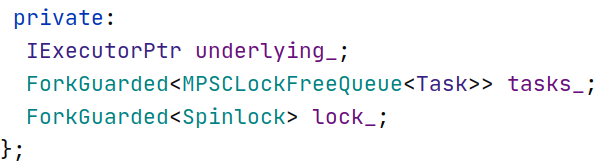
\includegraphics[scale=0.5]{forkguarded}}
	}
	\bigskip
	\caption{\mintinline{c++}{ForkGuarded<T>} в Strand-е.}
\end{figure}

\else

\begin{listing}
	\centering
	
	\begin{minted}{c++}
class Strand : public IExecutor {
// implementation...

private:
	IExecutorPtr executor_;
	ForkGuarded<MPSCLockFreeQueue<Task>> tasks_;
	ForkGuarded<Spinlock> lock_;
};
	\end{minted}
	\caption{\mintinline{c++}{ForkGuarded<T>} в Strand-е.}
	
\end{listing}

\fi


\section{Either / Random}

Чтобы перебрать больше сценариев в тесте, разветвлять можно и сам код. 

Для примера возьмем спинлок с методами \mintinline{c++}{Lock} и \mintinline{c++}{TryLock}. Естественный тест для него – это захват и освобождение лока в бесконечном цикле. У потока есть два варианта, как взять лок, и хочется проверить оба. В +Cal для этого есть конструкция \mintinline{c++}{either} / \mintinline{c++}{or}: она создает развилку в коде, в которой model checker пройдет по обеим веткам исполнения:

\begin{figure}
	\centerfloat{
		\fbox{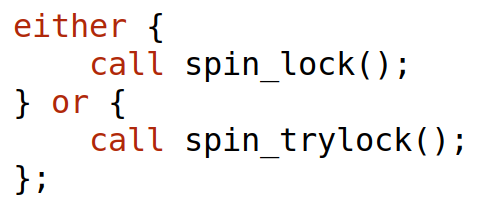
\includegraphics[scale=0.4]{caleither}}
	}
	\bigskip
	\caption{\mintinline{c++}{either} из +Cal.}
\end{figure}


В model checker-е для аналогичных целей реализована функция \mintinline{text}{bool Either()}. Вызов функции переключается на контекст model checker-а, и тот кладет в очередь состояний не один снимок, а два – каждый со своим выходом из \mintinline{c++}{Either}. Чтобы не создавать два почти одинаковых снимка состояния, model checker продолжает оба состояния еще на один шаг вперед. 

\iftoggleverb{pics}

%\begin{comment}
\begin{figure}
	\centerfloat{
		\fbox{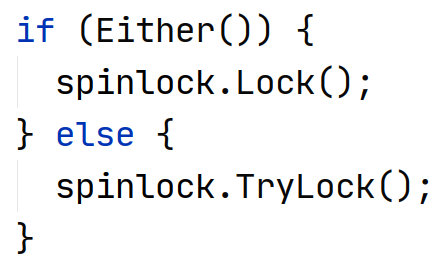
\includegraphics[scale=0.35]{either}}
	}
	\bigskip
	\caption{\mintinline{text}{Either} model checker-а.}
\end{figure}
%\end{comment}

\else

\begin{listing}
	\centering
	
	\begin{minted}{c++}
if (Either()) {
	lock.Lock();
} else {
	lock.TryLock();
}
	\end{minted}
	\caption{Тест для спинлока с Either.}
	
\end{listing}

\fi

Можно создавать не две, а произвольное число новых веток. Такая логика реализуется функцией \mintinline{text}{size_t Random(size_t n)}: она порождает $n$ новых продолжений, каждое с уникальным возвращаемым значением от $0$ до $n-1$. 

\mintinline{c++}{Random} позволяет писать тесты с более разнообразными сценариями исполнения. В +Cal-версии теста для LFAlloc поток всегда сначала аллоцирует узел, а потом возвращает обратно. Вместо этого поток может узнать, сколько узлов уже аллоцировано ($n$), и сгенерировать “случайное” значение с помощью \mintinline{c++}{Random(n+1)}. Если сгенерированное значение – $0$, поток аллоцирует еще один узел (вынимает из стека). Иначе – вызывает \mintinline{c++}{Free} на узле с полученным “случайным” индексом (возвращает в стек). Так потоки не будут привязаны к последовательности действий “\mintinline{c++}{Alloc} – \mintinline{c++}{Free} – \mintinline{c++}{Alloc} – \mintinline{c++}{Free} … “. Новому сценарию достаточно трех потоков вместо четырех для нарушения инварианта, время теста сокращается в шесть раз, а траектория получается короче – она не содержит лишних действий, появившихся из-за фиксированной структуры теста.

\iftoggleverb{pics}

\begin{figure}
	\centerfloat{
		\fbox{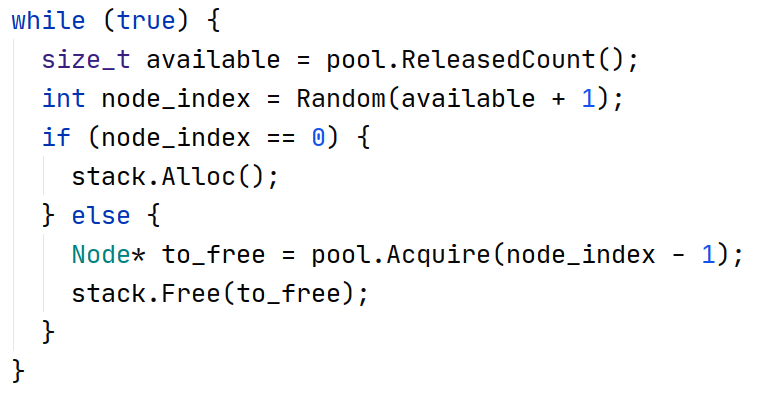
\includegraphics[scale=0.4]{stackrandom}}
	}
	\bigskip
	\caption{\mintinline{c++}{Random} в тесте lock-free стека.}
\end{figure}


\else

\begin{listing}
	\centering
	
	\begin{minted}{c++}
while (true) {
	size_t available = pool.ReleasedCount();
	int node_index = Random(available + 1);
	if (node_index == 0) {
		stack.Alloc();
	} else {
		Node* to_free = pool.Acquire(node_index - 1);
		stack.Free(to_free);
	}
}
	\end{minted}
	\caption{Random в тесте lock-free стека.}
	
\end{listing}

\fi 

Приведем окончательную статистику тестирования lock-free стека в LFAlloc:

\begin{table}
\centering
\begin{tabular}{| l | >{\bfseries}c | c | c |}
\hline
                              & \makecell{model checker \\ (с \mintinline{c++}{Random})}         & \makecell{model checker \\ (без \mintinline{c++}{Random})}  & TLC \\
                   \hline    
 Длина траектории             & 50 шагов                         & 61 шаг                      & 76 шагов \\ 
 Найдено состояний            & \numprint{2574023}               & \numprint{17906188}         & \numprint{26168885} \\      
 \makecell[l]{Найдено уникальных \\ состояний} & \numprint{789596}                & \numprint{4751588}          & \numprint{7269203} \\
 Время                        & 5 секунд                         & 29 cекунд                   & 8 минут\\
 	\hline
\end{tabular}

\bigskip
\captionsetup{justification=centering}
\caption{Статистика (с \mintinline{c++}{Random} и без) поиска ABA в LFAlloc.} 
\end{table}

Кроме того, функцию \mintinline{c++}{Random} использует сам model checker в реализации очереди ожидания в мьютексах и условных переменных: с помощью \mintinline{c++}{Random(n)} в \mintinline{c++}{WakeOne} он  может “недетерминированно” разбудить любой из $n$ спящих в очереди потоков.

\iftoggleverb{pics}

%\begin{comment}
	\begin{figure}
	\centerfloat{
		\fbox{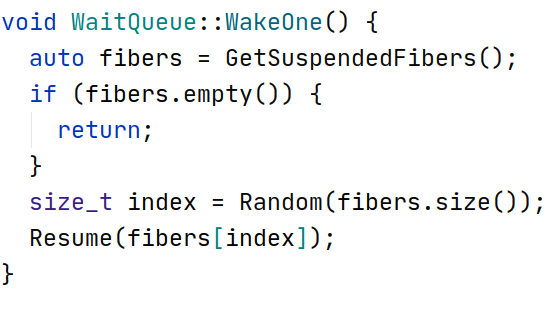
\includegraphics[scale=0.5]{wakeone}}
	}
	\bigskip
	\caption{\mintinline{c++}{Random} в реализации очереди ожидания.}
\end{figure}
%\end{comment}

\else

\begin{listing}
\centering

\begin{minted}{c++}
void WaitQueue::WakeOne() {
	auto fibers = GetSuspendedFibers();
	if (fibers.empty()) {
		return;
	}
	size_t index = Random(fibers.size());
	Resume(fibers[index]);
}
\end{minted}
\caption{Random в реализации очереди ожидания.}

\end{listing}

\fi


\section{Prune}

Служебная функция \mintinline{c++}{Prune} выбрасывает из рассмотрения текущее состояние.

\mintinline{c++}{Prune} можно использовать для проверки тестов с бесконечным графом исполнения. Например, мы хотим написать тест для ticket lock-а – но атомарный счетчик свободных билетов растет в нем бесконечно. Чтобы ограничить граф состояний, вызовем \mintinline{c++}{Prune} в местах, где билет становится больше какого-то порога: 

\iftoggleverb{pics}

\begin{figure}
	\centerfloat{
		\fbox{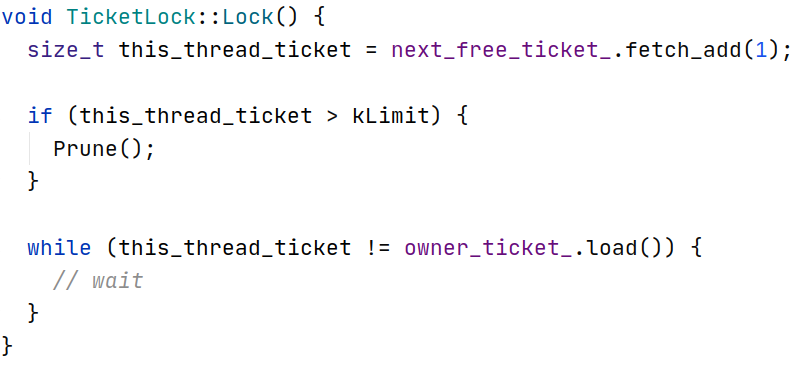
\includegraphics[scale=0.5]{prune}}
	}
	\bigskip
	\caption{\mintinline{c++}{Prune} в ticket lock.}
\end{figure}

\else

\begin{listing}
	\centering
	
	\begin{minted}{c++}
void TicketLock::Lock() {
	size_t this_thread_ticket = next_free_ticket_.fetch_add(1);

	if (this_thread_ticket > kLimit) {
		Prune();
	}

	while (this_thread_ticket != owner_ticket_.load()) {
		// wait
	}
}
	\end{minted}
	\caption{Prune в ticket lock.}
	
\end{listing}

\fi

Еще одно потенциальное применение \mintinline{c++}{Prune} – отсечение неперспективных веток исполнения для ускорения перебора.

\section{Детализация траектории}


\subsection{Заметки о событиях}

Подобно логированию, траекторию model checker-а можно детализировать заметками с помощью макроса \mintinline{c++}{SHOW_NOTE(message)}.

Заметки делятся на два типа:

\begin{itemize}
\item	Служебные – заметки, уже встроенные в атомики / примитивы синхронизации: результат чтения атомика, парковка потока на условной переменной, состояние очереди ожидания мьютекса. 

\begin{figure}
	\centerfloat{
		\fbox{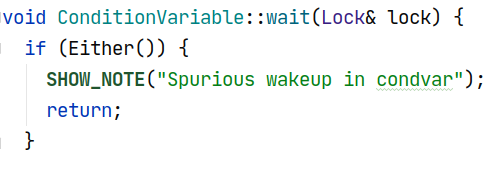
\includegraphics[scale=0.5]{spurcond}}
	}
	\bigskip
	\caption{Служебная заметка.}
\end{figure}

\item	Пользовательские – “отладочные” комментарии: поток зашел в определенную ветку кода, завершил какую-то операцию и т.п.

\begin{figure}
	\centerfloat{
		\fbox{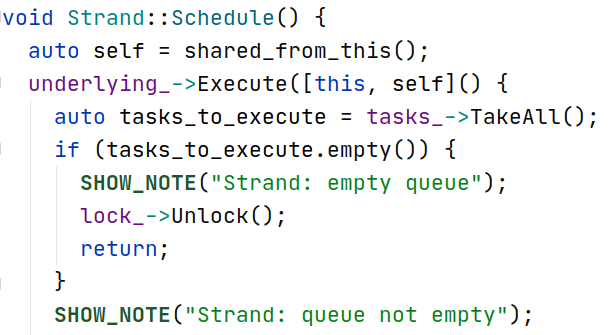
\includegraphics[scale=0.45]{shownote}}
	}
	\bigskip
	\caption{Пользовательские заметки.}
\end{figure}

\end{itemize}

\subsection{Описание разделяемого состояния}

При печати траектории model checker автоматически показывает стеки вызовов и состояние локальных переменных. Но об устройстве глобального состояния он ничего не знает.

Чтобы каждый “шаг” траектории сопровождался представлением разделяемого состояния, пользователь должен в начале теста передать функцию печати model checker-у с помощью вызова \mintinline{c++}{PrintState(std::function<StateDescription()>)}.

Описание задается в виде \mintinline{c++}{StateDescription} – объекта, который model checker уже умеет печатать (в json-подобном виде). \mintinline{c++}{StateDescription} строится инкрементально двумя способами:

\begin{itemize}
\item	передачей пары “ключ – значение”;

\item	передачей вложенного \mintinline{c++}{StateDescription}-а.
\end{itemize}

\iftoggleverb{pics}

\begin{figure}
	\centerfloat{
		\fbox{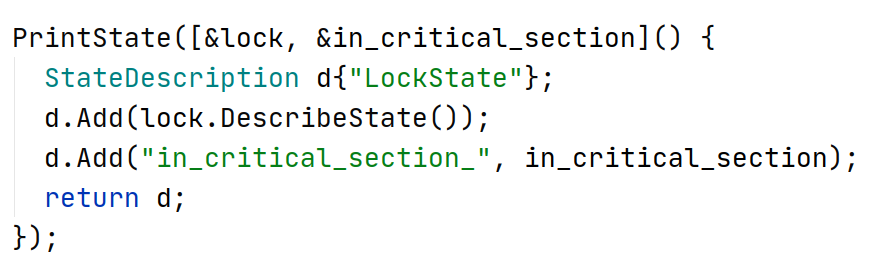
\includegraphics[scale=0.35]{descr}}
	}
	\bigskip
	\caption{Описание разделяемого состояния в тесте спинлока.}\label{fig:descr}
\end{figure}

\else

\begin{listing}
	\centering
	
	\begin{minted}{c++}
PrintState([&lock, &in_critical_section]() {
	StateDescription d{"LockState"};
	d.Add(lock.DescribeState());
	d.Add("in_critical_section_", in_critical_section);
	return d;
});
	\end{minted}
	\caption{Описание разделяемого состояния.}
	
\end{listing}

\fi
